% ------------ HEADER ------------ %


% PROJECT: Today I Learned Document
% AUTHOR: Miles Smith


% ------------ PREAMBLE  ------------ %


\documentclass[12pt]{article}
\usepackage{times}
\usepackage[margin=1in]{geometry}
\usepackage{amsmath,amsthm,amssymb}
\usepackage{graphicx}
\usepackage{multirow}
\usepackage{setspace}
\usepackage{subcaption}
\usepackage{caption}
\usepackage{float}
\doublespacing


% ------------ DOCUMENT ------------ %

\begin{document}

\begin{center}
\huge{\textbf{Today I Learned}}\\
\large{An insight into the fun things I am learning}\\

\vspace*{0.5cm}
\textbf{Miles Smith}\\

\vspace*{1cm}
\textbf{Introduction}\\
\textit{In an attempt to better document the things that I am learning and help things stick with me, I am hoping to create this running document so I can ramble about whatever cool things I learn each day.}\\
\vspace*{2cm}
\clearpage

\end{center}

\section{Tuesday, March 8, 2022}
\par
To continue on yesterday’s discussion about solid-state propulsion, Barrett’s group used a corona discharge thruster to propel the aircraft. This works by applying a DC voltage across two asymmetric electrodes as shown, where the positive electrode is a wire that ionizes air molecules within some radius, referred to as the corona (is this related to the Debye length?) and the negative electrode is some sort of mesh material. Ionized materials then move along the induced electric field and collide with neutral air molecules to produce in the opposite direction of ion flow. 

\begin{figure}[h]
\centering
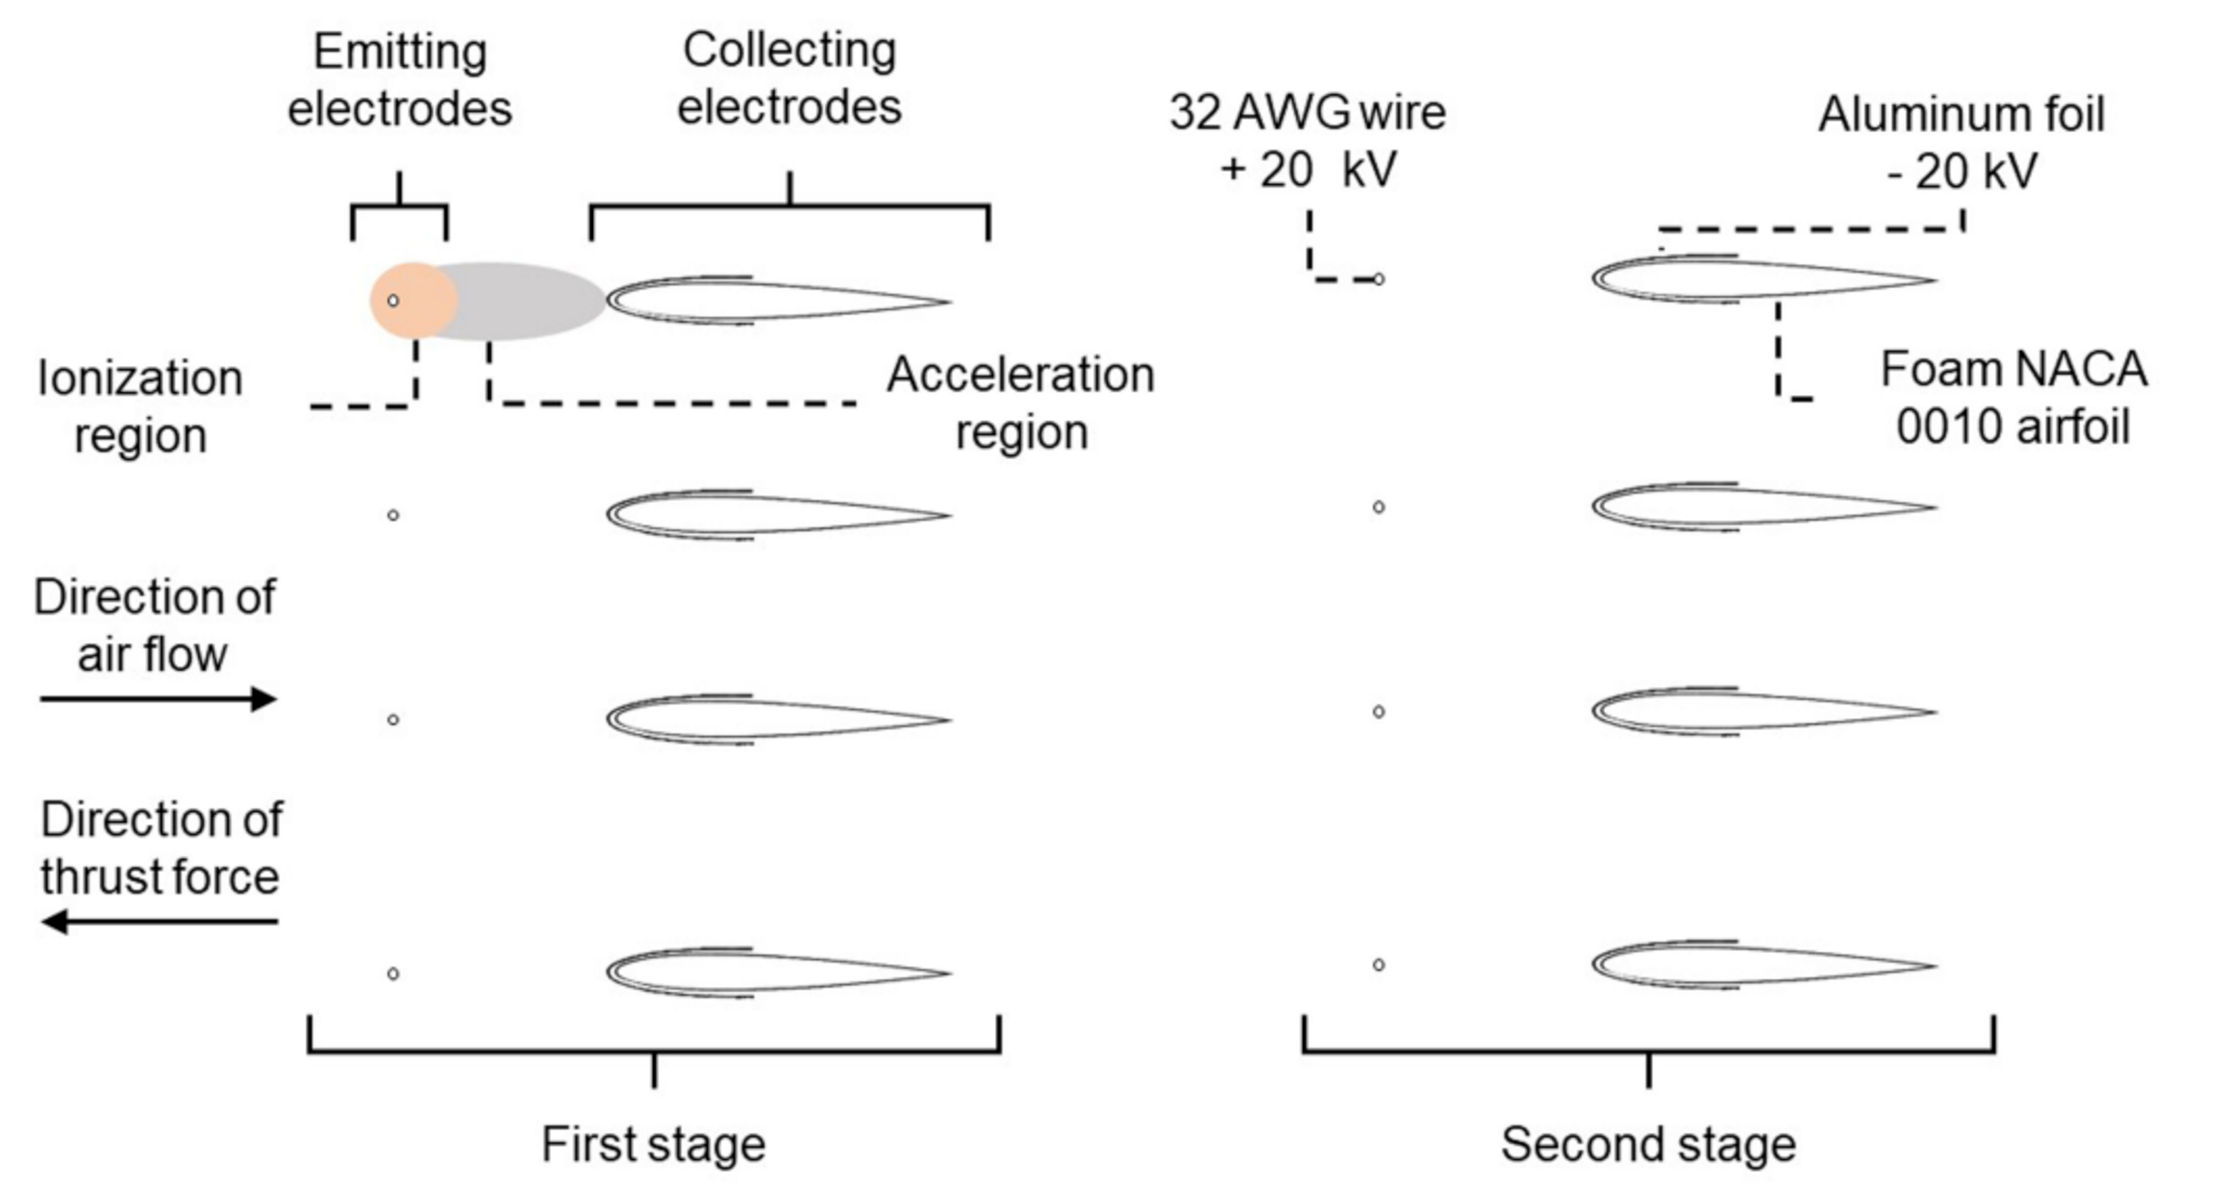
\includegraphics[width=\linewidth]{images/thrustdiagram.pdf}
\end{figure}

\section{Monday, March 7, 2022}
\par
An interesting topic that I was reading about today is “ionocraft” which are airplanes propelled by ion propulsion systems that have no moving parts. This article by Steven Barrett’s group shows a proof of concept on how a heavier than air craft can be propelled by ionic wind. From my understanding, it works by using high-voltage electrodes (20 kV+?) to ionize air (mostly N2) and accelerate the ions across the electric field to the negative electrode.  The thrust force is generated as a reaction to the motion of the ions. In their proof-of-concept tests, the craft traveled between 40-45 meters in 8-9s before turning the thruster off.

\begin{figure}[h]
\centering
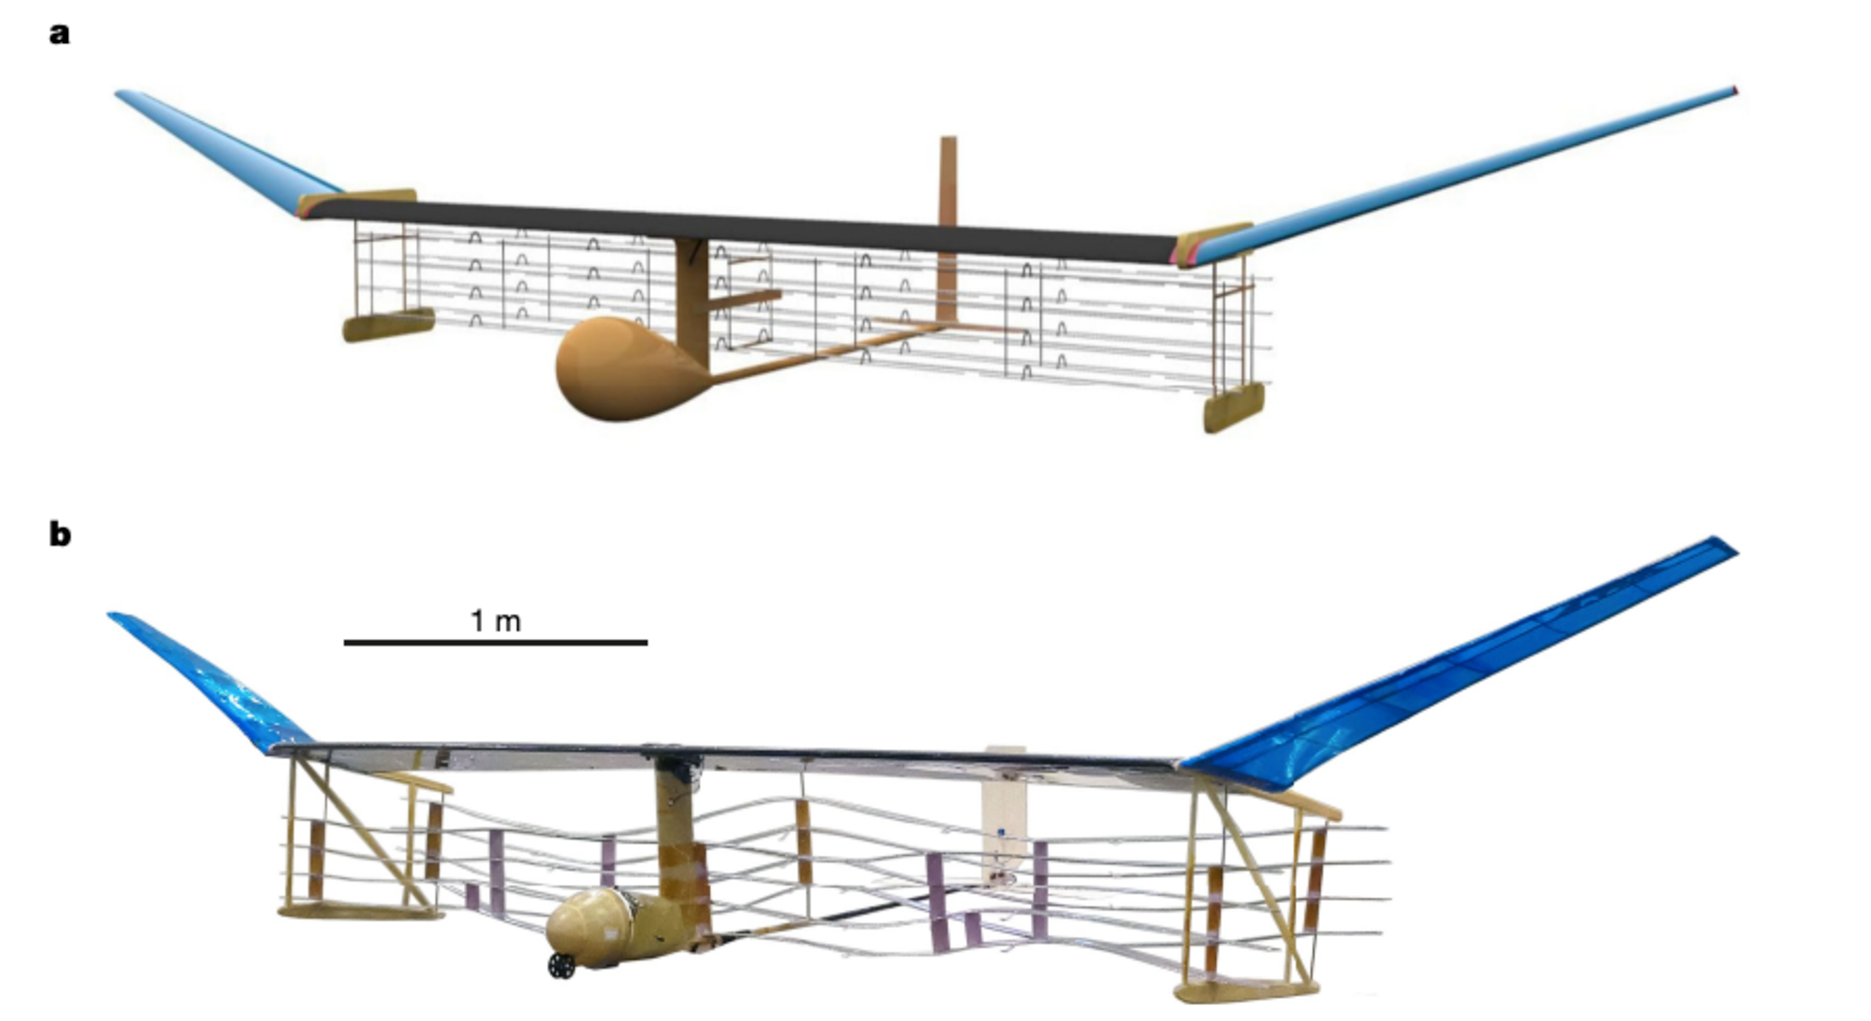
\includegraphics[width=\linewidth]{images/ionicwindplane.pdf}
\end{figure}

\begin{figure}[h]
\centering
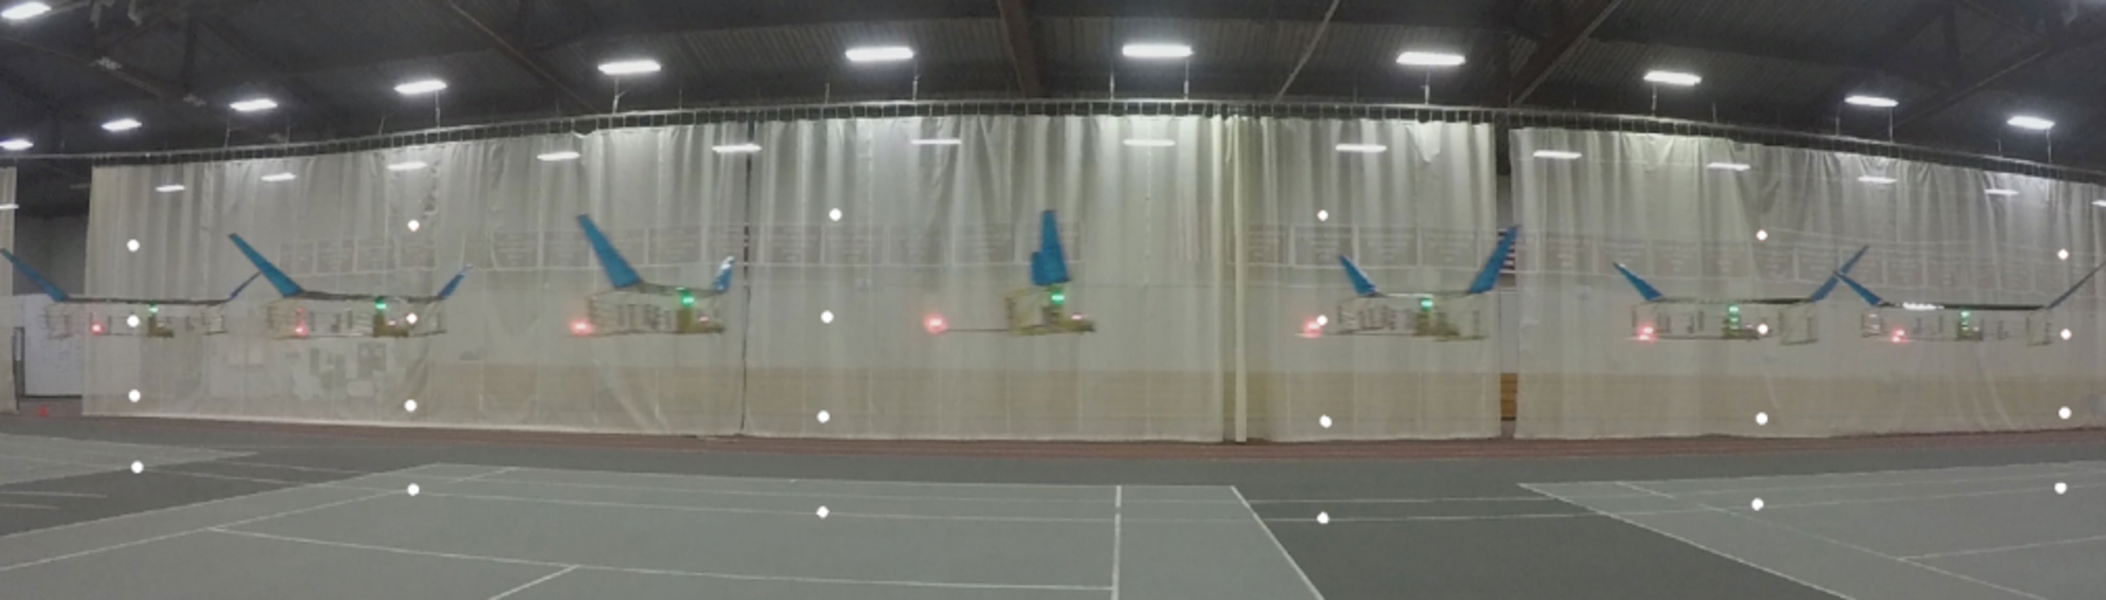
\includegraphics[width=\linewidth]{images/ionocraftmotion.pdf}
\end{figure}

\par
Today I also spent some time working on a computational fluid mechanics problem set for my Physics of Wind course. Given collected over a domain and assuming horizontally homogeneity I spatially averaged the data to study potential temperature and vertical velocity as a function of altitude in the atmospheric boundary layer. One part of the assignment involves applying similarity relationships to estimate the convective velocity scale and the surface heat flux, but I am not exactly sure how to do that. 



\end{document}